\subsection*{Question 4}

\noindent After running the tests on the selected packages with the selected mutations activated, we search for a class that has a lower mutation coverage. Since I was looking for mutants, I also searched for a class that has a high line coverage so I know that the mutants that survived were not simply not covered in order to learn more about mutants and how they work.\\ I found the class \verb|CharSequenceReader.java|

\begin{center}
        
\includegraphics[width=0.9\textwidth]{img/partD-before2.png}
\end{center}

\noindent Then I searched the class looking for some mutants that were not killed. 

\begin{center}
        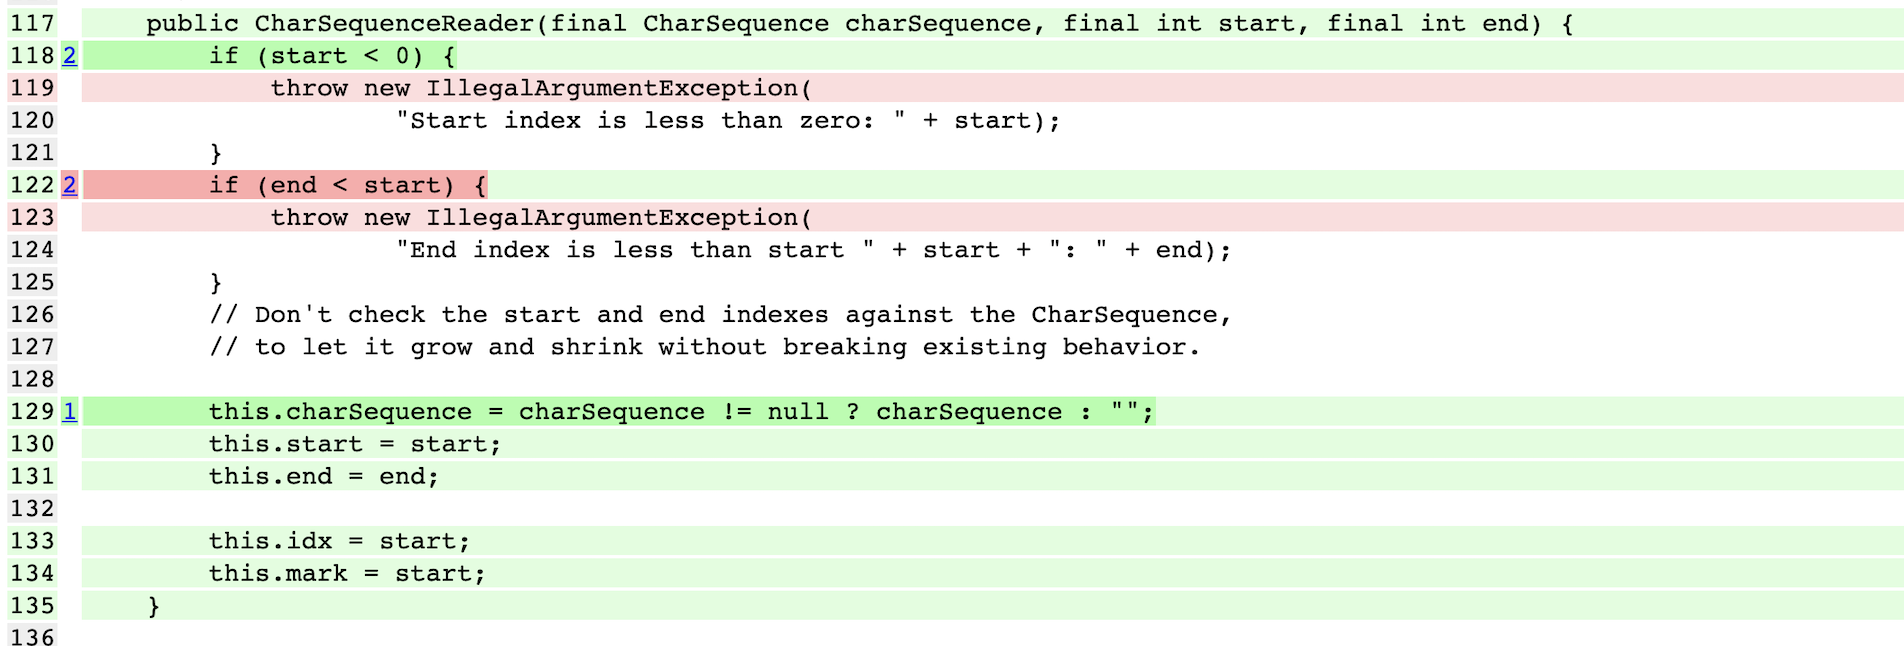
\includegraphics[width=0.9\textwidth]{img/partD-before3.png}
\end{center}

\noindent This \verb|CharSequenceReader| constructor has a series of if statement to verify if the \textit{start} and \textit{end} variables passed to it that specify respectively the start and end index in the character sequence to be read are logic. The first verifies if the start is not an negative integer. The second if is meant to verify that the end index is not smaller than the start. \\ The second if statement had a changed conditional boundary mutant that survived. Indeed, after taking a look at the tests that can be found in the \verb|CharSequenceReaderTest.java| file, I realized that no test handled the case where the start and end have the same value. I added a constructor and provided a start and end value of 2:
\begin{center}
        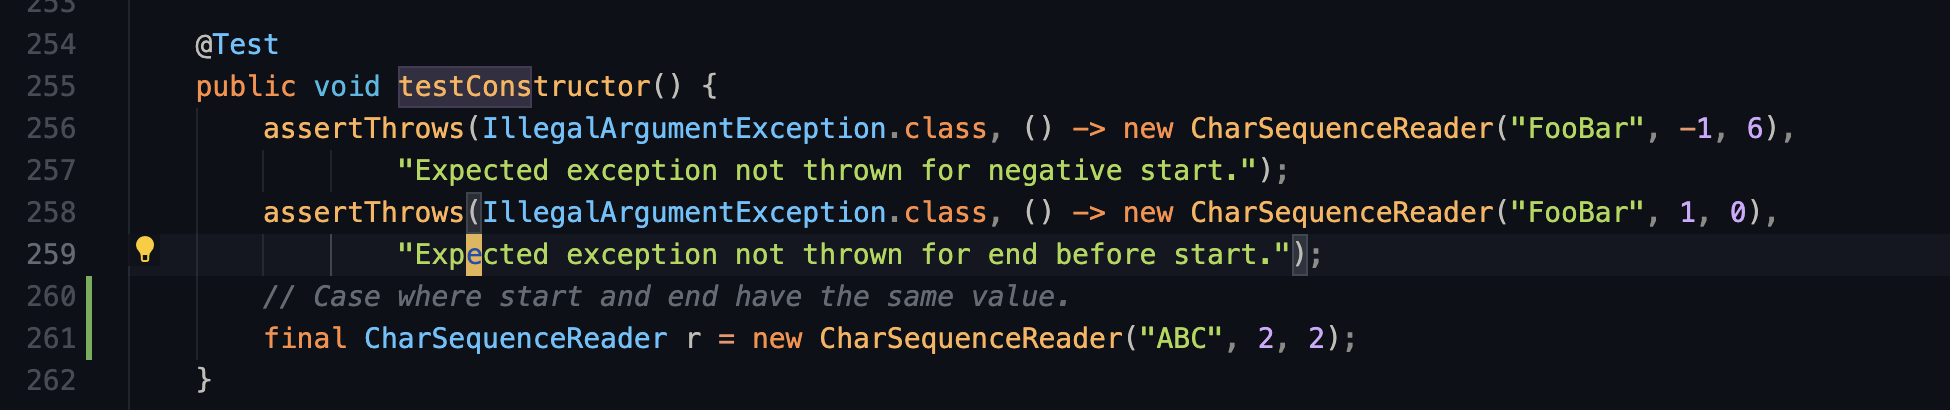
\includegraphics[width=0.9\textwidth]{img/partD-after.png}
\end{center}

\noindent After this addition, the result of the changed conditional boundary mutant would be different that that of the normal code. Indeed, while \verb|2 < 2| will return false, \verb|2 <= 2| will return true. The mutant was therefor killed and the mutation coverage and test strength meliorated. 

\begin{center}
        
\includegraphics[width=0.9\textwidth]{img/partD-after2.png}
        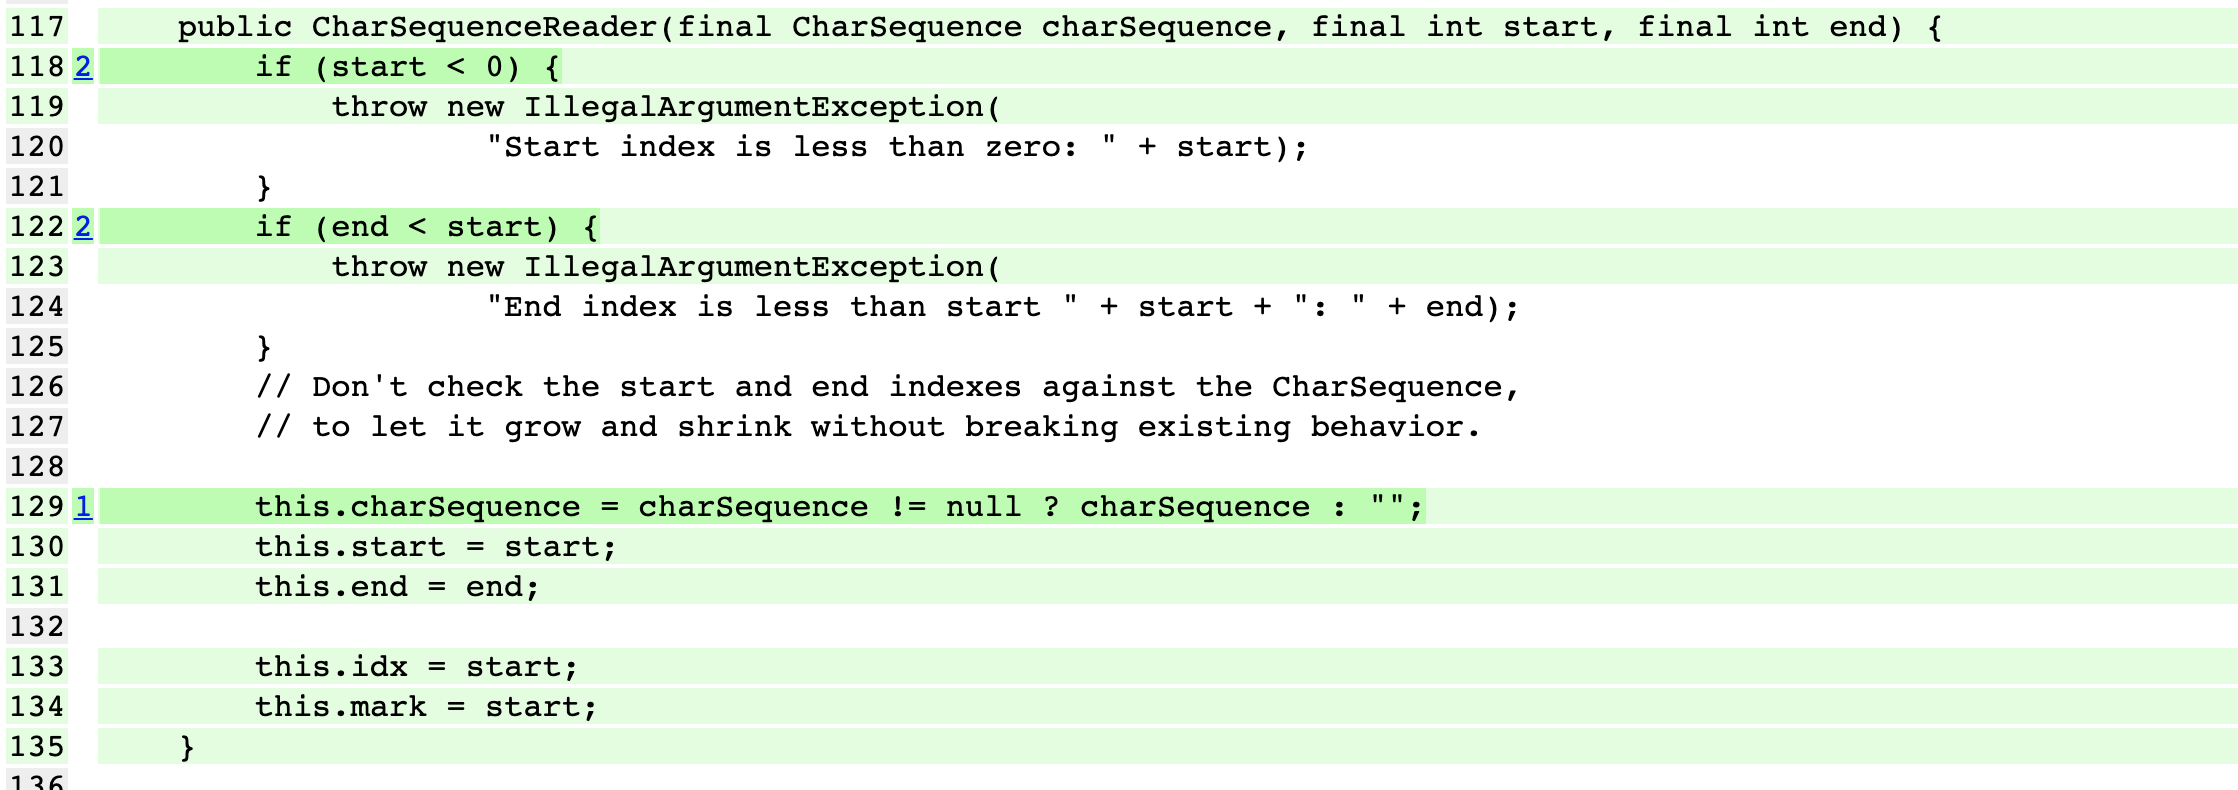
\includegraphics[width=0.9\textwidth]{img/partD-after3.png}
\end{center}